%!TEX program = xelatex

\documentclass[12pt]{article}
% \usepackage[utf8]{inputenc}
\usepackage[UTF8]{ctex}
\usepackage{indentfirst}
\usepackage{lmodern}% http://ctan.org/pkg/lm
\usepackage{setspace}
\usepackage{verbatim}
\usepackage{amsmath}%数学
\usepackage{amsthm}%数学定理、证明
\usepackage{graphicx}%graphicx基于graphics,更方便
% \usepackage{subfig}%图像
\usepackage{subfigure}
\usepackage{booktabs}%表格
\usepackage{tabularx}%表格
\usepackage{multirow}
\usepackage{multicol}
\usepackage{listings}
\usepackage{relsize}
\usepackage[usenames]{color}   
\usepackage{fontspec}
%更改页边距
\usepackage{geometry}
\geometry{left=2.0cm,right=2.0cm,top=2.5cm,bottom=2.5cm}

%并列图片
%\begin{figure}[H]
%	\begin{minipage}[t]{0.5\textwidth}
	%		\centering
	%		\includegraphics[width=0.8\textwidth]{img1}
	%		\caption{img1\label{fig:1}}
	%	\end{minipage}
%	\qquad
%	\begin{minipage}[t]{0.5\textwidth}
	%		\centering
	%		\includegraphics[width=0.8\textwidth]{img2}
	%		\caption{img2\label{fig:2}}
	%	\end{minipage}
%\end{figure}

%设置enumerate环境缩进两个字符
\usepackage{enumitem}
\setlist[enumerate]{listparindent=\parindent}

%更改enumerate编号样式
%\renewcommand{\labelenumi}{(\theenumi)}
%{\labelenumi}标明你要修改的那一级标签，如果是第2层，就是\labelenumii，以此类推；
%{(\theenumi)}用于表达你想要改成的标签式样，我是在原式样外面加括号，所以在\theenumi两边加了括号。其他参数的使用方法类似。

%\usepackage{colortbl}%表格颜色
\usepackage[table]{xcolor}
\usepackage{array}
\usepackage[rightcaption]{sidecap}
\usepackage{hyperref}
\usepackage{float}
\hypersetup{
	colorlinks=true,
	linkcolor=black
}%解决目录红框问题
\lstset{
 columns=fixed,       
 numbers=left,                                        % 在左侧显示行号
 numberstyle=\tiny\color{gray},                       % 设定行号格式
 frame=none,                                          % 不显示背景边框
 backgroundcolor=\color[RGB]{245,245,244},            % 设定背景颜色
 keywordstyle=\color[RGB]{40,40,255},                 % 设定关键字颜色
 numberstyle=\footnotesize\color{darkgray},           
 commentstyle=\it\color[RGB]{0,96,96},                % 设置代码注释的格式
 stringstyle=\rmfamily\slshape\color[RGB]{128,0,0},   % 设置字符串格式
 showstringspaces=false,                              % 不显示字符串中的空格
 breaklines=true,                                     % 对过长的代码自动换行
 language=python,                                     % 设置语言
}
\newcommand{\myd}{\;\mathrm{d}}%自定义积分变量命令
% \renewcommand{\listtablename}{表格}%改变listoftable的名字
\renewcommand{\arraystretch}{1.8}%The height of each row, relative to its default height
% \setmonofont{Consolas}
\renewcommand\refname{参考网站}
% \setlength{\tabcolsep}{18pt}%The space between the text and the left/right border of its containing cell
% \setlength{\arrayrulewidth}{0.4mm}%sets the thickness of the borders of the table

\setlength{\parindent}{2em}%控制首行缩进
\addtolength{\parskip}{3pt}%\parskip 控制段落(paragraph)距离
%\singlespacing%单倍行距
%\doublespacing%双倍行距
%\setstretch{1.25}%设置行距为1.25
\onehalfspacing %1.5倍行距
%\begin{doublespacing} 行距环境 \end{doublespacing}
\graphicspath{{./figures/}} % 指定图片所在文件夹
%\newtheorem{definition}[定义]{section}
%定制环境: {环境名}[编号延续]{显示名}[编号层次]
\newcommand{\daima}[1]{{\ttfamily{#1}}}

% 列表行间距
\usepackage{enumitem}
\setlist[itemize]{itemsep=-4pt}
\setlist[enumerate]{itemsep=-4pt}

% 表格宽度
\newcolumntype{H}{>{\centering\arraybackslash}p{2cm}}
\newcolumntype{C}{>{\centering\arraybackslash}p{2.4cm}}


\usepackage{algorithm2e}
\usepackage{amssymb}
\begin{document}
	\begin{titlepage}
		\vspace*{-2.5cm}
		\begin{figure}[h]
			\centering
			
\includegraphics[width=0.8\linewidth]{zjdx}
		\end{figure}
		\begin{figure}[h]
			\centering
			\includegraphics[width=0.3\linewidth]{QSY}
		\end{figure}
		\vspace{-0.2cm}
		\begin{center}
			\Huge{\textbf{基于CNN的MINIST手写数字识别}}\\
		\end{center}
		\vspace*{0.8cm}
		\begin{center}
			\larger[2]{
				\begin{tabular}{cc}
					姓\hspace{12pt}名 & \underline{\makebox[220pt]{\kaishu 黄鹤翔}}\\
					学\hspace{12pt}号 & \underline{\makebox[220pt]{3230106231}}\\
					院\hspace{12pt}系 & \underline{\makebox[220pt]{\kaishu 信息与电子工程学院}}\\
					指导老师 & \underline{\makebox[220pt]{\kaishu 赵明敏}}\\
				\end{tabular}
			}
		\end{center}
	\end{titlepage}
	\newpage
    \tableofcontents
	\newpage
	\pagenumbering{arabic}%重新开始标号,阿拉伯数字形式

\section{卷积神经网络理论}

\subsection{卷积神经网络的整体结构}
卷积神经网络是一种专门用于处理具有网格结构数据的深度学习模型，特别适用于图像识别任务。其整体结构通常包括以下几个主要部分：
\begin{itemize}
    \item 输入层：接受原始图像数据，通常以多维数组的形式表示。
    \item 卷积层：通过卷积操作提取图像的局部特征
    \item 池化层：降低特征图的空间维度，减少计算量，同时保留重要信息。
    \item 全连接层：将前面提取的高维特征展平后输入传统神经网络。
    \item 输出层：输出最终任务需要的指标
\end{itemize}
\begin{center}
    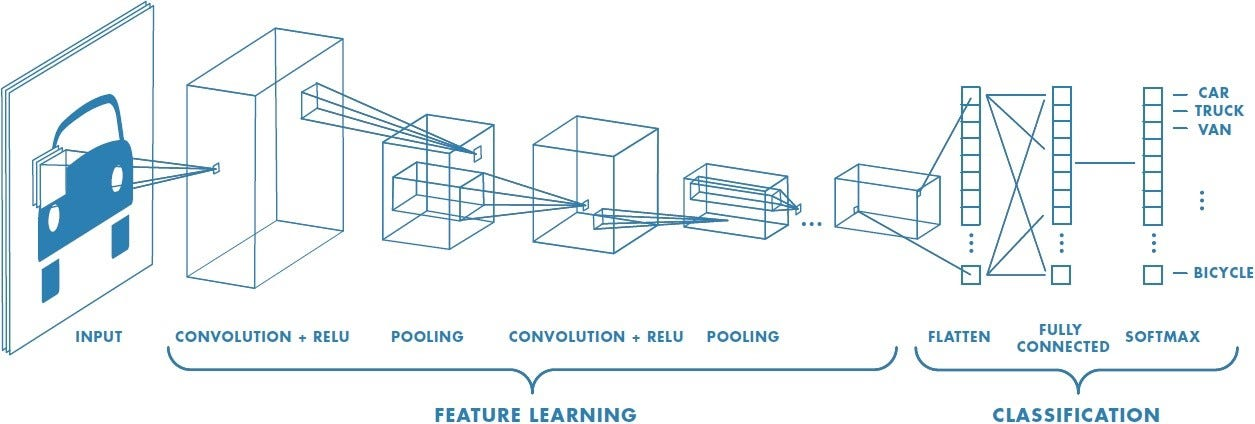
\includegraphics[scale = 0.3]{figures/cnn.jpg}
\end{center}

\subsection{卷积层}
\subsubsection{单通道卷积}
\begin{itemize}
    \item 输入为二维矩阵$X \in \mathbb{R}^{H \times W}$
    \item 卷积核为$K \in \mathbb{R}^{k \times k}$
    \item 输出特征图为$Y \in \mathbb{R}^{H' \times W'}$
\end{itemize}
则卷积运算定义为：
$$
Y[i, j] = \sum_{m=0}^{k-1} \sum_{n=0}^{k-1} X[i + m,\, j + n] \cdot K[m, n] + b
$$
其中，$b$为偏置项
\begin{center}
    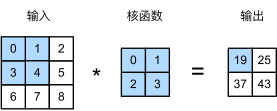
\includegraphics[scale = 0.5]{figures/single_conv.jpg}
\end{center}

\subsubsection{多通道卷积}
真实图像通常有多个输入通道（如 RGB 图像有 3 通道）。此时：
输入：$ X \in \mathbb{R}^{H \times W \times C_{\text{in}}} $
单个卷积核：$K \in \mathbb{R}^{k \times k \times C_{\text{in}}}$（必须与输入通道数一致）
对每个通道分别做卷积，然后相加，再加偏置：

$$
Y[i, j] = \sum_{c=1}^{C_{\text{in}}} \sum_{m=0}^{k-1} \sum_{n=0}^{k-1} X[i+m, j+n, c] \cdot K[m, n, c] + b
$$
若使用 $ C_{\text{out}} $ 个不同的卷积核，则输出为 $ Y \in \mathbb{R}^{H' \times W' \times C_{\text{out}}} $

\begin{center}
    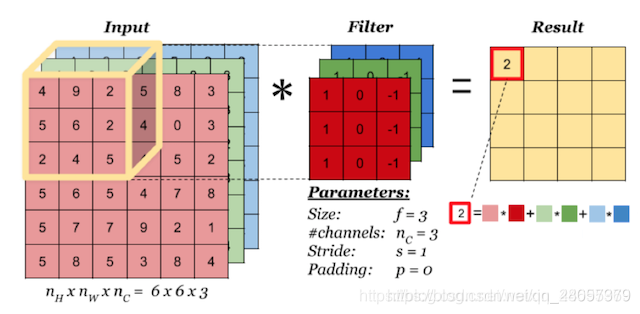
\includegraphics[scale = 0.5]{figures/multi_conv.png}
\end{center}
\begin{center}
    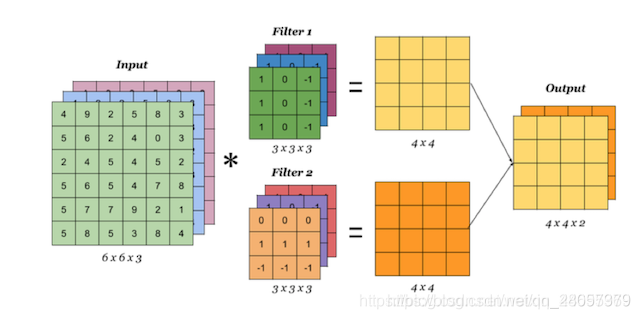
\includegraphics[scale = 0.5]{figures/multi_channal.png}
\end{center}

\subsection{池化层}
池化层（Pooling Layer）是卷积神经网络（CNN）中的一个关键组件，主要用于减少特征图的空间维度（宽度和高度），从而降低计算复杂度，并有助于控制过拟合。池化操作通常在卷积层之后进行，能够提取主要特征而忽略细节信息。
池化层主要有两种常见的操作方式：
\begin{itemize}
    \item 最大池化（Max Pooling）：在池化窗口内选择最大的值作为输出,以此来保留最显著的特征
    \item 平均池化（Average Pooling）：在池化窗口内计算平均,保留更多的背景信息，但可能丢失一些重要的特征
\end{itemize}
\begin{center}
    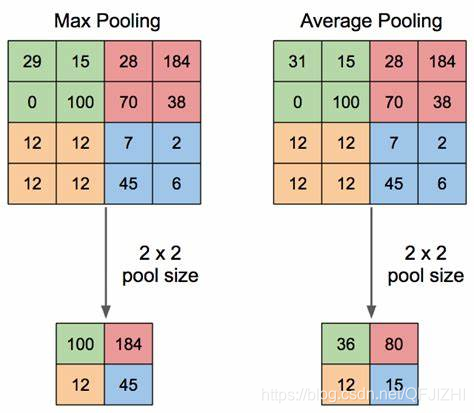
\includegraphics[scale = 0.5]{figures/pool.png}
\end{center}

\subsection{特征图大小计算}
\subsubsection{卷积层的特征图大小}
\textbf{符号定义}
\begin{center}
\begin{tabular}{c|c}
\hline
符号 & 含义 \\
\hline
$ H, W $ & 输入特征图的高度和宽度 \\
$ k $ & 卷积核（滤波器）的空间尺寸 \\
$ s $ & 步幅（stride） \\
$ p $ & 填充（padding），指在每一边添加的零像素数 \\
$ H', W' $ & 输出特征图的高度和宽度 \\
\hline
\end{tabular}
\end{center}

\textbf{输出尺寸公式}

$$
H' = \left\lfloor \frac{H + 2p - k}{s} \right\rfloor + 1
$$
$$
W' = \left\lfloor \frac{W + 2p - k}{s} \right\rfloor + 1
$$

\subsubsection{池化层的特征图大小}
池化操作（最大池化或平均池化）通常使用固定窗口（如 $2\times2$）和步幅（常等于窗口大小），不涉及填充（除非特别指定）。

\textbf{符号定义}

\begin{center}
\begin{tabular}{c|c}
\hline
符号 & 含义 \\
\hline
$ H, W $ & 池化层输入的高度和宽度 \\
$ f $ & 池化窗口大小\\
$ s $ & 池化步幅（通常 $s = f$） \\
$ p $ & 池化填充（一般为 0） \\
$ H_p, W_p $ & 池化后输出的高度和宽度 \\
\hline
\end{tabular}
\end{center}

\textbf{输出尺寸公式}

与卷积相同，池化本质上也是一种滑动窗口操作

$$
H_p = \left\lfloor \frac{H + 2p - f}{s} \right\rfloor + 1
$$
$$
W_p = \left\lfloor \frac{W + 2p - f}{s} \right\rfloor + 1
$$
\textbf{注：}实际中，池化通常无填充（$p = 0$），且 $s = f$（如 $2\times2$ 窗口，步幅为 2）。

\section{实验过程}
\subsection{实验数据获取}
本实验采用广泛使用的手写数字识别基准数据集——MNIST数据集。该数据集包含 60000 张训练图像和 10000 张测试图像，每张图像为 $28 \times 28$ 像素的灰度图，对应一个 0 到 9 的数字标签。\par

我们通过程序化方式从指定 URL 下载 MNIST 数据压缩包。具体实现如下：调用 download 工具函数从华为云 MindSpore 官方资源站点下载名为 \texttt{MNIST\_Data.zip} 的数据集文件，并自动解压至当前工作目录。相关代码如下所示：
\begin{lstlisting}
%env no_proxy='a.test.com,127.0.0.1,2.2.2.2'
from download import download
下载MNIST数据集
url = "https://mindspore-website.obs.cn-north-4.myhuaweicloud.com/" \
"notebook/datasets/MNIST_Data.zip"
path = download(url, "./", kind="zip", replace=True)
\end{lstlisting}
下载完成后，数据按标准格式组织为训练集（train/）与测试集（test/）两个子目录，便于后续加载与预处理。

\subsection{数据预处理}
为提升模型训练的稳定性与收敛速度，本实验对原始 MNIST 数据集进行了标准化的预处理流程。所有操作均通过 MindSpore 的 dataset 模块实现，以流水线（pipeline）方式高效处理图像与标签数据。具体预处理步骤如下：
\subsubsection*{图像尺寸调整（Resize）}
将原始 $28 \times 28$ 像素的灰度图像统一调整为 $32 \times 32$ 像素。采用双线性插值（Inter.LINEAR）方法进行上采样，以保留图像的平滑结构并适配后续可能引入的更大卷积网络结构（如 LeNet-5 常用 32×32 输入）。

\subsubsection*{像素值归一化（Rescale）}
将像素值从 $[0, 255]$ 的整型范围线性映射至 $[0, 1]$ 的浮点范围，即对每个像素执行 $x \leftarrow x / 255.0$。此操作将数据类型由 uint8 转换为 float32，便于后续数值计算。

\subsubsection*{Z-score 归一化（Normalize）}
使用 MNIST 数据集的全局统计参数（均值 $\mu = 0.1307$，标准差 $\sigma = 0.3081$）对图像进行 Z-score 归一化：
\[
x \leftarrow \frac{x - \mu}{\sigma}
\]
此步骤使输入数据分布接近标准正态分布，有助于加速模型收敛并提升泛化能力。

\subsubsection*{通道顺序转换（HWC2CHW）}
将图像张量从默认的 (Height, Width, Channel) 格式转换为深度学习框架常用的 (Channel, Height, Width) 格式（即 CHW），以满足卷积层的输入要求。

\subsubsection*{标签类型转换（TypeCast）}
将原始标签（通常为 int64 或 uint32）统一转换为 int32 类型，确保与损失函数和评估指标的输入要求兼容。

\subsubsection*{数据集划分与批处理}
在读取训练集时启用 shuffle=True，打乱样本顺序以避免训练过程中的周期性偏差；
使用 batch(batch\_size=32, drop\_remainder=True) 将数据划分为固定大小的小批量（mini-batch），并丢弃最后一个不足 32 样本的批次，保证每批次张量形状一致，提升训练效率。

相关代码如下所示：
\begin{lstlisting}
# 定义预处理操作的流程，整体对数据集进行处理
def datapipe(path, batch_size=32):
    image_transform = [
        # Resize： 以双线性插值方式调整图像尺寸大小
        vision.Resize(size=32, interpolation=Inter.LINEAR),
        # Rescale: 缩放图像的像素值大小，将像素值统一除255，数据类型由unit8转为float32
        vision.Rescale(1.0 / 255.0, 0.0),
        # Mormalize：将像素值归一化
        vision.Normalize(mean=(0.1307,),std=(0.3081,)),
        # HWC2CHW：将张量格式从（height,width,channel）转换成(channel,height,width)
        vision.HWC2CHW(),
        ]
    label_transform = transforms.TypeCast(ms.int32)
    # 利用MnistDataset接口读取解压后的MNIST的训练集和测试集，并进行shuffle操作
    dataset = MnistDataset(path, shuffle=True)
    # 通过map方法对每张图片应用数据处理操作
    dataset = dataset.map(operations=image_transform, input_columns=["image"])
    # 将每个标签的数据类型转换为int32
    dataset = dataset.map(operations=label_transform, input_columns=["label"])
    # 对数据集进行分批处理；当最后一个批处理数据包含的数据条目小于batch_size时，drop_remainder表示是否将该批处理丢弃，不传递给下一个操作。默认值：False，不丢弃。
    dataset = dataset.batch(batch_size, drop_remainder=True)
    return dataset

dataset_train = datapipe("MNIST_Data/train")
dataset_eval = datapipe("MNIST_Data/test")
\end{lstlisting}

\subsection{网络结构设计}
本实验中采用了经典的卷积神经网络架构 LeNet-5 作为手写数字识别模型，其网络结构设计如下：
\subsubsection*{输入层}
接收单通道灰度图像输入，尺寸为$32 \times 32$像素。
\subsubsection*{第一卷积层}
\begin{itemize}
\item 输入通道数：1
\item 输出通道数：6
\item 卷积核大小：$5 \times 5$
\item 填充大小：0
\end{itemize}
经过此层后，输出特征图尺寸变为$(32 - 2*0 + 5) / 1 + 1 = 28$，即$28 \times 28$，通道数为6。
之后使用ReLu激活函数进行非线性变换。
\subsubsection*{第一池化层}
采用$2 \times 2$的最大池化操作，步幅为2。
经过此层后，输出特征图尺寸变为$(28 - 2) / 2 + 1 = 14$，即$14 \times 14$，通道数仍为6。
\subsubsection*{第二卷积层}
\begin{itemize}
\item 输入通道数：6
\item 输出通道数：16
\item 卷积核大小：$5 \times 5$
\item 填充大小：0
\end{itemize}
经过此层后，输出特征图尺寸变为$(14 - 2*0 + 5) / 1 + 1 = 10$，即$10 \times 10$，通道数为16。
之后使用ReLu激活函数进行非线性变换。
\subsubsection*{第二池化层}
采用$2 \times 2$的最大池化操作，步幅为2。
经过此层后，输出特征图尺寸变为$(10 - 2) / 2 + 1 = 5$，即$5 \times 5$，通道数仍为16。
\subsubsection*{全连接层}
将池化层输出的特征图展平为一维向量，长度为$16 \times 5 \times 5 = 400$，并连接到包含120个神经元的全连接层与另一个包含84个神经元的全连接层。
激活函数选择ReLu。
\subsubsection*{输出层}
将全连接层的输出连接到一个包含10个神经元的输出层，对应手写数字的10个类别（0-9）。
\begin{center}
    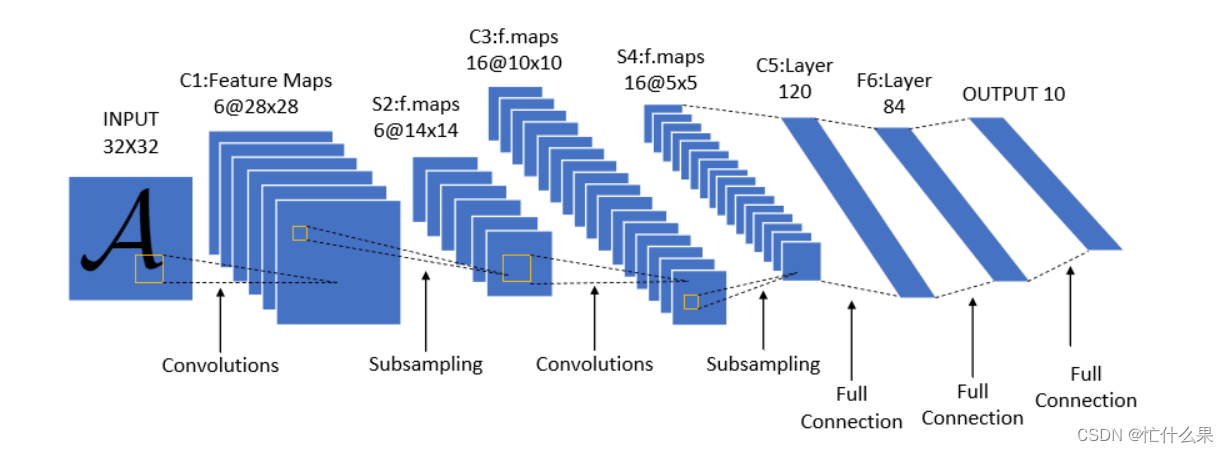
\includegraphics[scale = 0.3]{figures/lenet.png}
\end{center}
相关代码如下所示：
\begin{lstlisting}
#定义模型结构，MindSpore中的模型时通过construct定义模型结构，在__init__中初始化各层的对象
class LeNet5(nn.Cell):
    """LeNet5"""

    def __init__(self, num_classes=10, num_channel=1):
        super(LeNet5, self).__init__()
        # 卷积层，输入的通道数为num_channel,输出的通道数为6,卷积核大小为5*5
        self.conv1 = nn.Conv2d(num_channel, 6, 5, pad_mode='valid')
        # 卷积层，输入的通道数为6，输出的通道数为16,卷积核大小为5*5
        self.conv2 = nn.Conv2d(6, 16, 5, pad_mode='valid')
        # ReLU激活函数
        self.relu = nn.ReLU()
        # 池化层
        self.max_pool2d = nn.MaxPool2d(kernel_size=2, stride=2)
        # 多维数组展平为一维数组
        self.flatten = nn.Flatten()
        # 全连接层，输入个数为16*5*5，输出个数为120
        self.fc1 = nn.Dense(16 * 5 * 5, 120, weight_init=Normal(0.02))
        # 全连接层，输入个数为120，输出个数为84
        self.fc2 = nn.Dense(120, 84, weight_init=Normal(0.02))
        # 全连接层，输入个数为84，分类的个数为num_class
        self.fc3 = nn.Dense(84, num_classes, weight_init=Normal(0.02))

    def construct(self, x):
        # 使用定义好的运算构建前向网络
        x = self.conv1(x)
        x = self.relu(x)
        x = self.max_pool2d(x)
        x = self.conv2(x)
        x = self.relu(x)
        x = self.max_pool2d(x)
        x = self.flatten(x)
        x = self.relu(self.fc1(x))
        x = self.relu(self.fc2(x))
        x = self.fc3(x)
        return x
\end{lstlisting}

\subsection{训练过程}
\subsubsection{损失函数的选择}
手写数字识别本质上是一个多分类的问题，我们使用softmax激活函数与交叉熵损失函数\par
假设模型对一个样本的原始输出（logits）为向量
$$
\mathbf{z} = (z_1, z_2, \dots, z_C) \in \mathbb{R}^C
$$
其中 $C$ 是类别数，真实标签为 one-hot 向量 $\mathbf{y} = (y_1, \dots, y_C)$（或整型类别索引）。

损失函数为：
$$
\mathcal{L} = -\sum_{i=1}^{C} y_i \log\left( \text{Softmax}(z_i) \right)
= -\sum_{i=1}^{C} y_i \log\left( \frac{e^{z_i}}{\sum_{j=1}^{C} e^{z_j}} \right)= -z_{\text{true}} + \log\left( \sum_{j=1}^{C} e^{z_j} \right)
$$
\subsubsection{优化器选择}
在深度学习中，优化器（Optimizer） 负责根据损失函数的梯度更新模型参数，以最小化损失。优化器的类型主要有：
\begin{itemize}
    \item SGD（随机梯度下降）：最基本的优化器，使用固定学习率更新参数。
    \item Momentum：在 SGD 基础上增加动量项，能够加速收敛并减少振荡。
    \item Adam：结合了 RMSProp 和 Momentum 的优点，使用自适应学习率和动量，通常收敛速度较快。
\end{itemize}
在本实验中我们选择了Momentum优化器，其更新公式为：
$$
v_t = \beta v_{t-1} + (1 - \beta) \nabla L(\theta_t)
$$
$$
\theta_{t+1} = \theta_t - \alpha v_t
$$
其中，$v_t$ 是动量项，$\beta$ 是动量衰减率（通常取 0.9），$\alpha$ 是学习率，$\nabla L(\theta_t)$ 是当前参数 $\theta_t$ 的梯度。
\subsubsection{训练流程与训练代码}
首先实例化 LeNet5 网络；
定义损失函数为 SoftmaxCrossEntropyWithLogits（适用于多分类任务）；
选用 Momentum 优化器，学习率设为 0.01，动量系数为 0.9，并传入模型所有可训练参数。\par

在训练过程中利用 mindspore.value\_and\_grad 自动计算损失对模型参数的梯度；
在每个 batch 中执行前向传播 → 计算损失 → 反向求导 → 参数更新。
每完成一个 epoch 的训练后，在测试集上评估模型性能，
遍历整个测试集，计算平均损失和分类准确率。\par

总共训练 100 个 epoch；
每个 epoch 结束后立即保存模型检查点（.ckpt 文件），便于后续加载或断点续训。\par

相关代码如下所示：
\begin{lstlisting}
network = LeNet5()

# 定义损失函数
net_loss = nn.SoftmaxCrossEntropyWithLogits(sparse=True, reduction='mean')
# 定义优化器，通过model.trainable_params()方法获得模型的可训练参数，并传入学习率超参来初始化优化器
net_opt = nn.Momentum(network.trainable_params(), learning_rate=0.01, momentum=0.9)

# 定义用于训练的train_loop函数。
def train_loop(model, dataset, loss_fn, optimizer):
    # 定义正向计算函数
    def forward_fn(data, label):
        logits = model(data)
        loss = loss_fn(logits, label)
        return loss

    # 定义微分函数，使用mindspore.value_and_grad获得微分函数grad_fn,输出loss和梯度。
    # 由于是对模型参数求导,grad_position 配置为None，传入可训练参数。
    grad_fn = ms.value_and_grad(forward_fn, None, optimizer.parameters)

    # 定义 one-step training函数
    def train_step(data, label):
        loss, grads = grad_fn(data, label)
        optimizer(grads)
        return loss

    size = dataset.get_dataset_size()
    model.set_train()
    for batch, (data, label) in enumerate(dataset.create_tuple_iterator()):
        loss = train_step(data, label)

        if batch % 100 == 0:
            loss, current = loss.asnumpy(), batch
            print(f"loss: {loss:>7f}  [{current:>3d}/{size:>3d}]")

# 定义用于测试的test_loop函数。
def test_loop(model, dataset, loss_fn):
    num_batches = dataset.get_dataset_size()
    model.set_train(False)
    total, test_loss, correct = 0, 0, 0
    for data, label in dataset.create_tuple_iterator():
        pred = model(data)
        total += len(data)
        test_loss += loss_fn(pred, label).asnumpy()
        correct += (pred.argmax(1) == label).asnumpy().sum()
    test_loss /= num_batches
    correct /= total
    print(f"Test: \n Accuracy: {(100*correct):>0.1f}%, Avg loss: {test_loss:>8f} \n")

epochs = 100
for t in range(epochs):
    print(f"Epoch {t+1}\n-------------------------------")
    train_loop(network, dataset_train, net_loss, net_opt)
    ms.save_checkpoint(network, "./save_direct.ckpt")
    test_loop(network, dataset_eval, net_loss)
print("Done!")
\end{lstlisting}

\subsection{模型验证}
为验证训练后 LeNet-5 模型在手写数字识别任务上的实际性能，本实验从测试集中随机选取一批样本进行推理，并通过可视化方式直观展示预测结果。
相关代码如下所示：
\begin{lstlisting}
# 将模型参数存入parameter的字典中，采用load_checkpoint接口加载模型参数
param_dict = ms.load_checkpoint("./save_direct.ckpt")
# 重新定义一个LeNet5神经网络
net = network
# 将参数加载到网络中
ms.load_param_into_net(net, param_dict)
model = Model(net)
data_test = dataset_eval.create_dict_iterator()
data = next(data_test)
images = data["image"].asnumpy()
labels = data["label"].asnumpy()

# 使用函数model.predict预测image对应分类
output = model.predict(ms.Tensor(data['image']))
pred = np.argmax(output.asnumpy(), axis=1)

plt.figure()
for i in range(1, 9):
    plt.subplot(2, 4, i)
    plt.imshow(images[i-1].squeeze(), cmap="gray")
    plt.title(pred[i-1])
plt.show()
\end{lstlisting}

\newpage
\section{实验数据与数据分析}
\subsection{预处理数据}
图像数据预处理之后的图像数据与图片为：
\begin{center}
    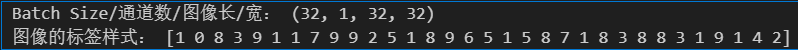
\includegraphics[scale = 0.5]{figures/img_size.png}
\end{center}
\begin{center}
    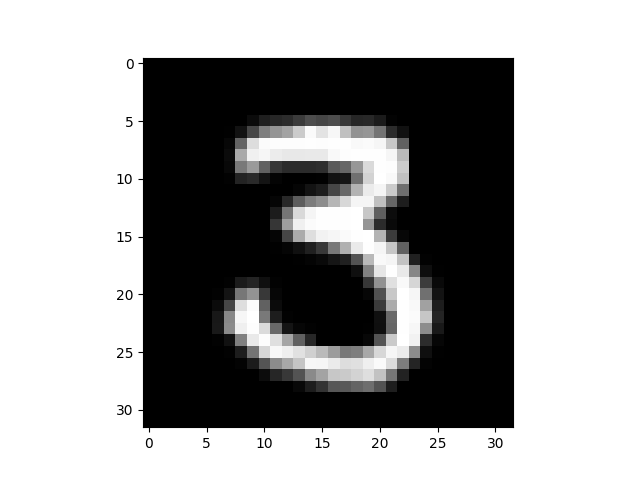
\includegraphics[scale = 0.5]{figures/mnist_sample.png}
\end{center}
通过上面的输出可以知道图像已经被处理到如下结构，满足图像预处理目标
\begin{itemize}
    \item 每批包含 32 张图像
    \item 图像为单通道灰度图
    \item 原始 28×28 图像已通过 vision.Resize(32) 成功上采样变为 32×32 图像
    \item 张量格式已成功转换为 (Channel, Height, Width)
    \item 标签为整形
\end{itemize}
\subsection{训练过程数据}
每个epoch训练集损失曲线和测试集准确率曲线如下：
\begin{center}
    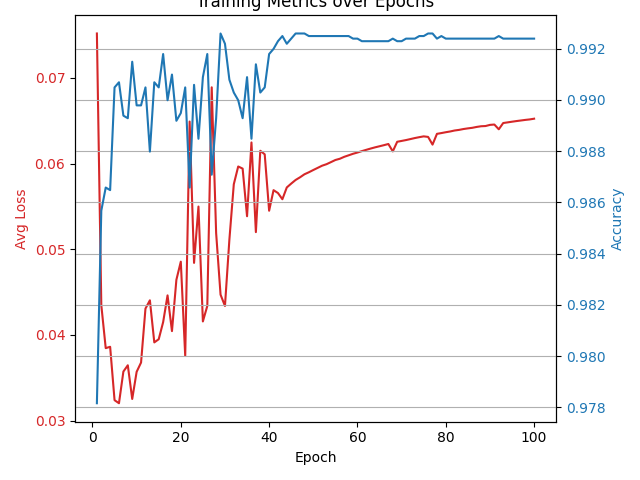
\includegraphics[scale = 0.8]{figures/metrics_plot.png}
\end{center}
\subsubsection*{整体收敛性分析}
\begin{itemize}
    \item 训练损失初始训练时大幅下降，表明模型在训练集上逐渐学习到有效特征，收敛性良好
    \item 测试准确率曲线整体上升，最终达到较高水平，说明模型具有良好的泛化能力。
    \item 训练后期损失缓慢上升,说明模型对极少数难样本（如笔画模糊或结构异常的数字）产生了高置信度错误预测，导致损失增大,但还是保持在较低的水平,且准确度较高,不影响模型的有效性
\end{itemize}
\subsubsection*{关键性能指标}
\begin{itemize}
    \item 最终测试准确率高于 99.0\%，符合预期的手写数字识别性能
    \item 收敛所需的epoch约为30轮
    \item 训练损失下限为0.03,模型拟合程度较好
\end{itemize}
\subsubsection*{训练效率与稳定性评估}
\begin{itemize}
    \item 早期收敛速度较快,说明学习率和优化器选择较为合理
    \item 后期波动幅度较小,最后 20 轮准确率标准差 < 0.2\%,训练稳定
\end{itemize}
\subsection{验证数据}
在测试集中取出八张图进行验证,均正确识别了手写数字
\begin{center}
    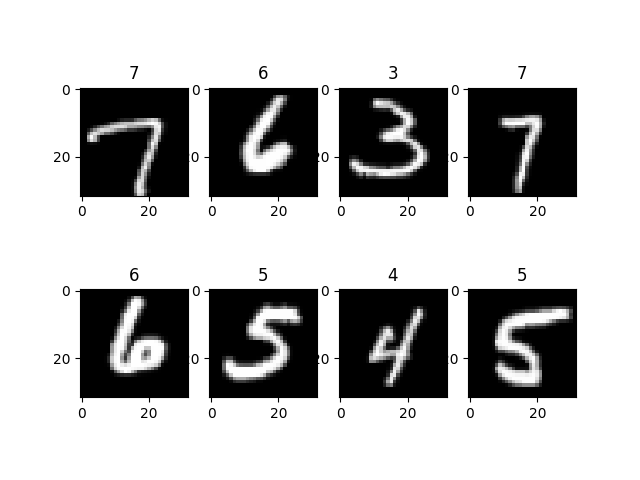
\includegraphics[scale = 0.8]{figures/recognize_result.png}
\end{center}

\section{训练改进}
\subsection{网络结构修改}
为了达到更高的准确率，我在网络中额外添加了一层卷积层，修改后网络与效果如下
\begin{lstlisting}
#定义模型结构，MindSpore中的模型时通过construct定义模型结构，在__init__中初始化各层的对象
class LeNet5(nn.Cell):
    """LeNet5"""

    def __init__(self, num_classes=10, num_channel=1):
        super(LeNet5, self).__init__()
        # 卷积层，输入的通道数为num_channel,输出的通道数为6,卷积核大小为5*5
        self.conv1 = nn.Conv2d(num_channel, 6, 5, pad_mode='valid')
        # 卷积层，输入的通道数为6，输出的通道数为16,卷积核大小为5*5
        self.conv2 = nn.Conv2d(6, 16, 5, pad_mode='valid')
        # 新增卷积层，输入的通道数为16，输出的通道数为32,卷积核大小为3*3
        self.conv3 = nn.Conv2d(16, 32, 3, pad_mode='valid')
        # ReLU激活函数
        self.relu = nn.ReLU()
        # 池化层
        self.max_pool2d = nn.MaxPool2d(kernel_size=2, stride=2)
        # 多维数组展平为一维数组
        self.flatten = nn.Flatten()
        # 全连接层，输入个数为32*4*4，输出个数为120
        self.fc1 = nn.Dense(32 * 4 * 4, 120, weight_init=Normal(0.02))
        # 全连接层，输入个数为120，输出个数为84
        self.fc2 = nn.Dense(120, 84, weight_init=Normal(0.02))
        # 全连接层，输入个数为84，分类的个数为num_class
        self.fc3 = nn.Dense(84, num_classes, weight_init=Normal(0.02))

    def construct(self, x):
        # 使用定义好的运算构建前向网络
        x = self.conv1(x)
        x = self.relu(x)
        x = self.max_pool2d(x)
        x = self.conv2(x)
        x = self.relu(x)
        x = self.conv3(x)
        x = self.relu(x)
        x = self.max_pool2d(x)
        x = self.flatten(x)
        x = self.relu(self.fc1(x))
        x = self.relu(self.fc2(x))
        x = self.fc3(x)
        return x
\end{lstlisting}
\begin{center}
    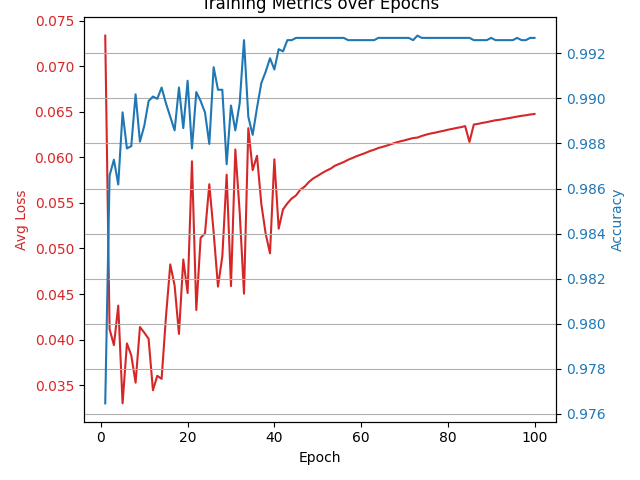
\includegraphics[scale = 1.0]{多卷积层.png}
\end{center}
\begin{itemize}
    \item 可以发现准确率与loss值在收敛后并无显著变化，同时收敛所需的轮数有略微的提升，添加卷积层并未带来明显的性能提升，反而增加了计算复杂度
\end{itemize}

\subsection{超参数修改}
观察训练过程的准确率与loss值，我发现模型大概在50轮之后开始收敛，之后loss值开始缓慢上升，说明模型在训练集上过拟合，泛化能力下降。针对这一问题，我加入了早停机制，当验证集准确率变化不大时，loss值变化小于阈值0.001时，停止训练，避免过拟合。\par
同时注意到模型在训练中期有震荡现象，猜测是学习率过大导致的，为了进一步提升模型性能，我对训练的学习率进行了动态调整，引入余弦退火的学习率衰减策略。
$$
    \eta_t = \eta_{\min} + \frac{1}{2}(\eta_{\max} - \eta_{\min}) \left(1 + \cos\left(\frac{T_{\text{cur}} \pi}{T_{\text{max}}}\right)\right)
$$

\begin{itemize}
    \item $\eta_{\max}$：初始的最大学习率(\texttt{0.01})。
    \item $\eta_{\min}$：最终的最小学习率(\texttt{0.001})。
    \item $T_{\text{cur}}$：当前的训练步数或 Epoch。
    \item $T_{\text{max}}$：总的训练步数或 Epoch。
\end{itemize}
\begin{lstlisting}
lr = nn.cosine_decay_lr(min_lr=0.001, max_lr=0.01, total_step=epochs*steps_per_epoch, step_per_epoch=steps_per_epoch, decay_epoch=epochs)
\end{lstlisting}
引入如上策略后的训练曲线如下：
\begin{center}
    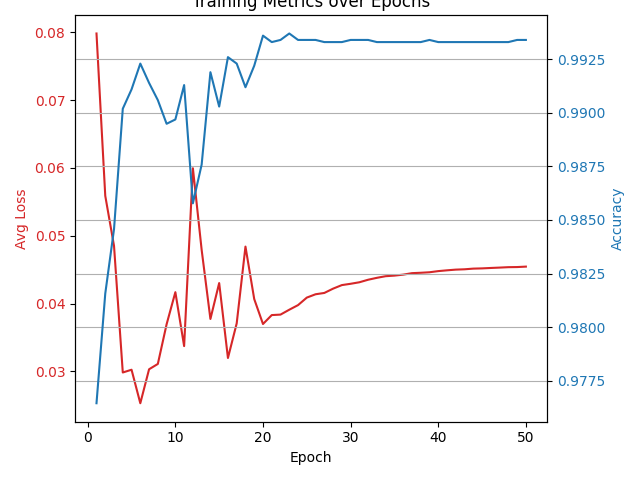
\includegraphics[scale = 0.8]{退火学习率.png}
\end{center}
从图像中我们可以发现模型有如下进步，说明上述改进是有效的：
\begin{itemize}
    \item 模型的震荡现象显著减小
    \item 模型的收敛速度有明显提升，从50轮缩短至30轮
    \item 最终的准确率有小幅提升
\end{itemize}
\section{实验总结}
通过本次实验，我们成功实现了一个端到端的手写数字识别系统。从可视化的训练曲线可以看出，模型的损失值随着训练轮次的增加而稳定下降，同时准确率稳步提升，表明模型有效地从数据中学习到了区分不同数字的特征。最终的预测结果也证实了该CNN模型对于MNIST手写数字具有很高的识别准确率。

此次实践不仅加深了我们对卷积神经网络工作原理的理解，也完整地体验了使用MindSpore框架进行深度学习项目开发的标准流程，包括数据处理、模型定义、训练、评估、可视化及推理等关键环节，为后续更复杂的计算机视觉任务奠定了坚实的基础。
\end{document}